% Revised project report.  Compile with XeLaTeX (Bengali text needs fontspec):
%   cd report && xelatex report.tex && xelatex report.tex
\documentclass[10pt,a4paper,twocolumn]{article}
\usepackage[margin=1.9cm,columnsep=0.7cm]{geometry}
\usepackage{fontspec}
\setmainfont{Times New Roman}
\newfontfamily\bengalifont[Script=Bengali,Scale=0.95]{Nirmala UI}
\newcommand{\bn}[1]{{\bengalifont #1}}
\usepackage{amsmath,booktabs,graphicx,array,multirow,xcolor,caption,microtype}
\usepackage{tikz}\usetikzlibrary{arrows.meta,positioning}
\usepackage[round]{natbib}
\usepackage[colorlinks=true,linkcolor=blue!50!black,citecolor=blue!50!black,urlcolor=blue!50!black]{hyperref}
\captionsetup{font=small,labelfont=bf}
\setlength{\tabcolsep}{4pt}
\newcommand{\best}[1]{\textbf{#1}}

\title{\vspace{-1.2cm}\textbf{Knowledge Graph-Based Automated Short Answer Grading for Bengali}\\[2pt]
\large NLP Dominator}
\author{Sourav Nath (2025201054) \quad Diganta Sen (2025201050) \quad Kushal Mukherjee (2025201072)\\[2pt]
International Institute of Information Technology, Hyderabad\\[2pt]
\small\textbf{Code:} \url{https://github.com/DigantaSen/Knowledge-Graphs-Based-Bengali-Answer-Evaluation}\\
\small\textbf{Models:} \url{https://huggingface.co/k040902/bengali_question_ans}}
\date{}

\begin{document}
\maketitle

\begin{abstract}
Automated short answer grading (ASAG) for Bengali is hampered by free word
order, agglutinative morphology and the lack of labelled data and of a
Bengali dependency parser. Similarity-only systems give near-perfect scores
to answers whose roles are swapped (\emph{Karak reversal}) or that are
negated. We present a Bengali ASAG system that combines LaBSE similarity with
(1)~a predicate-centred knowledge graph compared by a Siamese graph attention
network, (2)~a Karak (semantic-role) validator, (3)~negation, number and
\emph{answer-slot} features that compare only the part of an answer that
answers the question, and (4)~an XGBoost\,+\,MLP scorer trained with
synthetic error examples. We evaluate on three datasets of increasing answer
length with grouped splits, calibrated baselines and bootstrap confidence
intervals. On normal answers the system reaches Pearson 0.83 / 0.95 / 0.91
(single / medium / long) against 0.63 / 0.92 / 0.79 for the best baseline,
with significant MAE reductions on all three, and it scores hand-written
role-swapped and negated answers at 0--18 instead of 50--90. We also report
that the original datasets are heavily templated: a model trained on them
alone scores natural medium-length answers worse than a baseline (Pearson
0.20 vs 0.74), which a small, rubric-scored clean synthetic dataset fixes.
\end{abstract}

\section{Introduction}
Automatic grading of short factual answers underpins intelligent tutoring and
large-scale assessment. Progress has been strong for English
\citep{mohler2011,sultan2016,riordan2017}, but Bengali, spoken by over 230
million people, is harder: \emph{free word order} lets subject, object and
verb appear in almost any order; \emph{fused grammatical markers} (case
endings such as \bn{-কে}, negation fused into verbs such as \bn{হয়নি}) defeat
exact token matching; and there is no production-quality dependency parser.

Multilingual sentence encoders such as LaBSE \citep{labse} and BanglaBERT
\citep{banglabert} are a strong baseline, but sentence similarity is
insensitive to structure. A student who writes \bn{রাবণ রামকে বধ করেছিলেন}
(``Ravana killed Rama'') when the reference is \bn{রাম রাবণকে বধ করেছিলেন}
shares every content word with it, yet is completely wrong. We call this
failure mode \emph{Karak reversal}, after the Sanskrit-derived concept of
semantic roles (\emph{karak}) in Bengali grammar. Negated answers
(\bn{সূর্য পূর্বদিকে ওঠে না}) and wrong numbers or places are similar blind
spots. Our contributions are:
\begin{enumerate}\setlength{\itemsep}{0pt}
\item A Bengali ASAG pipeline with a predicate-centred knowledge graph and
  Siamese GAT, a Karak validator that handles case-marked objects and
  passives, sentence-aligned negation and number checks, and answer-slot
  features (\S\ref{sec:method}).
\item An audit of the three datasets: duplicated pairs with conflicting
  scores, overlapping label bands and pervasive answer templates, with a
  grouped, deduplicated evaluation protocol (\S\ref{sec:data}).
\item A rubric-scored clean synthetic dataset (514 rows, 54 new questions)
  and synthetic training errors, which expose and remove a template shortcut
  (\S\ref{sec:clean}).
\item An evaluation with calibrated baselines, bootstrap confidence intervals,
  unseen-question splits, an adversarial set and a component ablation.
\end{enumerate}

\section{Related Work}
\paragraph{Automated short answer grading.}
Early ASAG combined lexical overlap with dependency alignment;
\citet{mohler2011} showed that dependency-tree alignment beats bag-of-words
but relies on a parser that does not exist for Bengali. \citet{sultan2016}
used token alignment with paraphrase resources; neural models help under low
resources \citep{riordan2017,horbach2017}. None of these distinguish a
sentence from its Karak-reversed form when word order is free.

\paragraph{Models and Bengali tools.}
LaBSE \citep{labse} is trained contrastively on 109 languages; BanglaBERT
\citep{banglabert} is an ELECTRA discriminator. We found BanglaBERT
mean-pooled word vectors unusable for word similarity (every pair of Bengali
words has cosine $\geq 0.82$), so LaBSE is used for words and graph nodes.
Graph attention networks \citep{gat} outperform GCNs \citep{gcn} on
dependency-aware tasks \citep{zhang2019}. For Bengali structure the tooling
gap is severe: Stanza \citep{stanza} has no Bengali model; Trankit
\citep{trankit} lists Bengali only as trainable, and the only Universal
Dependencies treebank (BRU) has fewer than 1,000 units; the multilingual
triple extractor mREBEL \citep{mrebel} covers 18 languages without Bengali;
IndIE \citep{indie} was evaluated on Hindi; BanglaAutoKG \citep{banglaautokg}
builds corpus-level graphs with an LLM and untyped edges. We therefore build
per-answer, typed graphs from BNLP POS tags with rules.

\section{Data}\label{sec:data}
\subsection{Base datasets}
Three datasets pair a question, a reference answer and a student answer with
a score (0--100) and a label: \emph{single-sentence} (1,000 rows),
\emph{medium} (1,000 rows, 2--3-sentence references) and \emph{long} (320
rows, paragraphs). Our audit (Table~\ref{tab:data}) found four problems that
affect evaluation:
\begin{itemize}\setlength{\itemsep}{0pt}
\item \textbf{Few questions}: 50 per dataset (16 for long), one reference each.
\item \textbf{Duplicates}: 331 (single) and 508 (medium) rows repeat an earlier
  (reference, student) pair, and 193 of 200 repeated groups carry different
  scores. With a random row split, 47\% (single) and 73\% (medium) of test
  rows had an identical pair in training.
\item \textbf{Overlapping label bands}: e.g. single-sentence \emph{incorrect}
  answers reach 40 while \emph{partially correct} starts at 35.
\item \textbf{Templates}: a recurring 3-word prefix or suffix that never occurs
  in a reference (e.g.\ \bn{এই প্রশ্নের উত্তরে}, \bn{আরও তথ্য প্রয়োজন।},
  \bn{আজ রবিবার।}) appears in 53 single, \textbf{695} medium and 113 long
  student answers and largely determines the score.
\end{itemize}
We merge identical (question, reference, student) rows, averaging their
scores, and split by identical pair (``unseen answers'') or by question
(``unseen questions'').

\begin{table}[t]
\centering\small
\begin{tabular}{lrrr}
\toprule
 & Single & Medium & Long \\
\midrule
Rows (raw) & 1000 & 1000 & 320 \\
Questions & 50 & 50 & 16 \\
Repeated pairs & 331 & 508 & 29 \\
After deduplication & 669 & 492 & 291 \\
Templated answers & 53 & 695 & 113 \\
Correct band & 85--100 & 85--100 & 78--100 \\
Partial band & 35--80 & 40--75 & 25--77 \\
Incorrect band & 0--40 & 5--35 & 0--26 \\
\midrule
Train / test (normal) & 568 / 101 & 418 / 74 & 247 / 44 \\
Synthetic train rows & 111 & 125 & 74 \\
\bottomrule
\end{tabular}
\caption{Dataset statistics. Label bands are the observed score ranges per label. Every test set also contains the 51 adversarial samples.}
\label{tab:data}
\end{table}

\subsection{Adversarial samples}
We hand-wrote 51 adversarial samples, used for testing only: Karak reversal
(17; \bn{বিড়াল ইঁদুর ধরেছে} $\rightarrow$ \bn{ইঁদুর বিড়ালকে ধরেছে}),
negation (17), wrong number (4; 206 $\rightarrow$ 205 bones), wrong location
(2), partial cover (1, scored 50) and voice change (10; the active reference
rewritten as a passive with the roles reversed, \bn{পোরাসের দ্বারা
আলেকজান্ডার পরাজিত হয়েছেন}). All but partial cover are scored 0.

\subsection{Synthetic training errors}
Because adversarial samples never appear in training, a scorer cannot learn
that such answers score 0. We therefore add rule-generated errors to the
\emph{training split only}: each reference sentence is negated (\bn{না} after
the final verb, \bn{নয়} after a nominal predicate), its subject and
\bn{-কে} object are swapped, or its first number is changed by one, and an
unchanged copy is added so that short pairs are not all wrong. Synthetic rows
are capped at 30\% of the real training rows, and sentences used by the
adversarial samples are excluded.

\subsection{Clean synthetic dataset}\label{sec:clean}
To test whether the system grades natural answers rather than templates, we
wrote a second dataset of 514 rows for 54 new questions (30 single, 16
medium with three key facts each, 8 long with five). Each student answer has
a declared type and its score comes from a fixed rubric, not human graders:
for single sentences, copy 100, paraphrase 95, correct passive or other
construction 92, extra correct detail 92, brief key answer 88, partial 55,
key right but a detail wrong 40, wrong entity 10, wrong detail 8, and role
swap, negation, off-topic or ``don't know'' 0. For medium and long answers each
key fact is worth $95/k$ points and a contradicted fact costs a further 10.
Labels use non-overlapping bands ($\geq$85 correct, 35--84 partial). The rows
are marked \texttt{source=clean\_synthetic}; we report them separately.

\section{Method}\label{sec:method}
Figure~\ref{fig:arch} shows the pipeline.

\begin{figure}[t]
\centering
% System architecture (TikZ) — included by report.tex
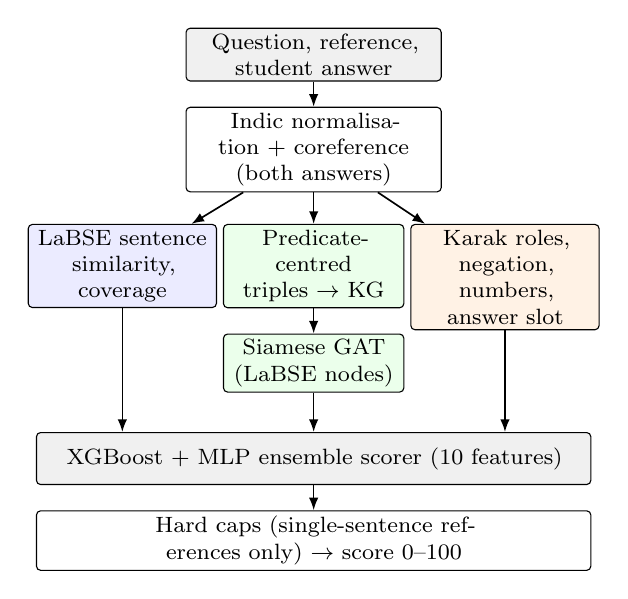
\begin{tikzpicture}[
  font=\footnotesize, node distance=3.2mm and 2.6mm,
  box/.style={draw, rounded corners=1.5pt, align=center, minimum height=6.6mm, inner sep=2pt, fill=#1},
  box/.default=white,
  arr/.style={-{Latex[length=1.6mm]}, semithick}]
\node[box=gray!12, text width=3.1cm] (in) {Question, reference, student answer};
\node[box, below=of in, text width=3.1cm] (pre) {Indic normalisation +\ coreference (both answers)};
\node[box=blue!8, below left=4mm and -4mm of pre, text width=2.25cm] (sem) {LaBSE sentence\ similarity, coverage};
\node[box=green!8, below=4mm of pre, text width=2.15cm] (kg) {Predicate-centred\ triples $\rightarrow$ KG};
\node[box=orange!10, below right=4mm and -4mm of pre, text width=2.25cm] (rule) {Karak roles, negation,\ numbers, answer slot};
\node[box=green!8, below=of kg, text width=2.15cm] (gnn) {Siamese GAT\ (LaBSE nodes)};
\node[box=gray!12, below=5mm of gnn, text width=6.9cm] (sc) {XGBoost + MLP ensemble scorer (10 features)};
\node[box, below=of sc, text width=6.9cm] (ov) {Hard caps (single-sentence references only) $\rightarrow$ score 0--100};
\draw[arr] (in) -- (pre);
\draw[arr] (pre) -- (sem); \draw[arr] (pre) -- (kg); \draw[arr] (pre) -- (rule);
\draw[arr] (kg) -- (gnn);
\draw[arr] (sem.south) -- (sem.south |- sc.north); \draw[arr] (gnn) -- (sc); \draw[arr] (rule.south) -- (rule.south |- sc.north);
\draw[arr] (sc) -- (ov);
\end{tikzpicture}

\caption{System architecture. Coreference is applied to both answers; three feature groups feed a learned ensemble, followed by hard caps for single-sentence references.}
\label{fig:arch}
\end{figure}

\paragraph{Normalisation and coreference.}
Text is normalised with the Indic NLP library. A rule-based resolver replaces
whole-token pronouns (\bn{তিনি}, \bn{এটি}, \ldots) with the most recent
proper noun (persons) or common noun (things), seeded from the reference
first because the question contains the interrogative, not the answer. It is
applied to both answers so that a verbatim copy stays a copy.

\paragraph{Roles from POS tags.}
BNLP's tagger emits the BIS tagset (\texttt{NC}, \texttt{NP}, \texttt{VM},
\ldots), mapped to universal POS. A rule parser labels the first unmarked
nominal as subject, \bn{-কে}-marked nominals as explicit objects, other
nominals after the subject as unmarked objects, the nominal before
\bn{দ্বারা}/\bn{কর্তৃক} as the agent of a passive (whose grammatical subject
becomes the patient), and genitive and locative nominals by explicit
endings. Lemmas strip case endings (\bn{রামকে} $\rightarrow$ \bn{রাম}).

\paragraph{Predicate-centred knowledge graph.}
Each clause becomes \emph{subject} $\xrightarrow{\text{agent}}$
\textsc{predicate} $\xrightarrow{\text{object/location/time/count}}$
\emph{argument}, with genitives attached to the noun they modify and
adjectives as qualities. The predicate node carries the verb, the noun of a
compound verb (\bn{বধ করেছিলেন}) and any negation (\bn{ওঠে না}); proper-noun
runs and number+unit are merged into single nodes. Node features are the
LaBSE embedding of the node text plus a one-hot node type and a negation flag
(775 dimensions); edge features are the weight, a one-hot relation type and a
direction flag, with reverse edges added.

\paragraph{Siamese GAT.}
Two GATv1 layers (4 heads, 256 $\rightarrow$ 128 dimensions, edge features of
dimension 9) with layer normalisation and mean pooling embed each graph; the
cosine of the two embeddings is regressed onto score/100 (MSE, Adam, lr
0.005, 5 epochs, batch 32, seeded).

\paragraph{Karak validator.}
Roles are compared per aligned sentence pair (sentences paired by token
overlap). A swap is counted only when the student marks the moved entity
explicitly (\bn{-কে} or passive patient): a reference agent that appears as a
marked object, or a reference object that becomes the subject while the
subject changes, adds 0.5. Identical inflected words in another order are a
legal reordering and exempt. Missing locations, numbers and modifiers and a
negation mismatch add smaller penalties (capped at 1).

\paragraph{Negation, numbers and entities.}
Negation is detected on punctuation-stripped tokens, including fused
\bn{-নি} forms, and compared per aligned sentence pair. A wrong number is a
digit run in the student answer that the reference lacks. Entity mismatch is
the share of reference content words (plus NER entities) missing from the
student answer, with LaBSE similarity $\geq 0.85$ counting as a synonym
(measured: synonyms 0.84--0.98, different entities 0.31--0.83).

\paragraph{Answer-slot features.}
Words that also occur in the question are shared by right and wrong answers
alike. Removing them leaves the \emph{answer content}, from which we compute
its recall and precision between reference and student, and
\emph{key\_match}: whether the key answer item is present (the number for
\bn{কবে}/\bn{কত}, the place or direction for \bn{কোথায়}, the item named by
\bn{কোন X}, else the first proper noun, skipping titles such as \bn{সম্রাট}).

\paragraph{Scorer and overrides.}
Ten features (LaBSE similarity, graph similarity, Karak penalty, entity
mismatch, sentence coverage, negation and wrong-number flags, and the three
answer-slot features) plus twelve products and differences feed XGBoost (300
trees, depth 5) and an MLP (128-64-32). The scorer is trained on
\emph{out-of-fold} GNN similarities so that it sees unseen-row values, and the
XGBoost/MLP weight is chosen on out-of-fold training predictions. For
single-sentence references only, a negation mismatch caps the score at 30
and a wrong number at 25 (fixed rules); multi-sentence answers receive partial
credit from human graders, so there the flags are left to the scorer.

\section{Experimental Setup}
Splits hold out 15\% of groups (identical pairs, or questions) with seed 42;
the 51 adversarial samples are always test-only. Baselines map a single
similarity to the score scale with a linear regression fitted on the training
split: LaBSE cosine, ROUGE-L (with a Bengali tokenizer), LaBSE\,+\,ROUGE-L,
BanglaBERT cosine (with its official normaliser) and the GNN alone. We report
Pearson correlation, MAE, the share of answers within $\pm$10 points, and
binary F1 of the pass class (score $\geq$ 50); 95\% confidence intervals and
$p$-values come from a paired bootstrap (2,000 resamples) of the proposed
system against the best baseline (lowest MAE). Cross-validation uses five
grouped folds over all normal rows, with a fresh GNN and scorer per fold.
Everything runs on a CPU; a full run of all three datasets with
cross-validation takes about 25 minutes.

\section{Results}

\begin{table*}[t]
\centering\small
\begin{tabular}{lccc|ccc|ccc}
\toprule
 & \multicolumn{3}{c|}{Single-sentence (n=152)} & \multicolumn{3}{c|}{Medium (n=125)} & \multicolumn{3}{c}{Long (n=95)} \\
Model & Pearson & MAE & F1 & Pearson & MAE & F1 & Pearson & MAE & F1 \\
\midrule
LaBSE cosine & 0.306 & 30.26 & 55.0 & 0.028 & 32.68 & 50.8 & 0.108 & 35.57 & 37.4 \\
ROUGE-L & 0.514 & 26.14 & 54.9 & 0.279 & 27.73 & 54.7 & 0.234 & 31.78 & 46.2 \\
LaBSE + ROUGE-L & 0.436 & 28.35 & 61.7 & 0.246 & 28.38 & 55.7 & 0.133 & 34.79 & 40.4 \\
BanglaBERT cosine & 0.241 & 32.00 & 48.4 & 0.225 & 30.10 & 54.2 & 0.296 & 32.67 & 56.7 \\
GNN only & 0.442 & 27.10 & 52.9 & 0.308 & 28.47 & 63.7 & 0.347 & 32.21 & 48.8 \\
\textbf{Proposed} & \best{0.830} & \best{12.10} & \best{80.4} & \best{0.855} & \best{9.49} & \best{86.0} & \best{0.788} & \best{12.19} & \best{72.3} \\
\bottomrule
\end{tabular}
\caption{Full test sets (normal + 51 adversarial rows), unseen-answer split. Baselines are linearly calibrated on the training split. The pooled numbers mix two populations; Table~\ref{tab:normal} reports normal answers alone.}
\label{tab:full}
\end{table*}

\begin{table*}[t]
\centering\small
\resizebox{\textwidth}{!}{%
\begin{tabular}{llcccccc}
\toprule
Dataset (n) & Best baseline & Baseline P / MAE & Proposed Pearson [95\% CI] & Proposed MAE [95\% CI] & $\Delta$Pearson ($p$) & $\Delta$MAE ($p$) & CV Pearson \\
\midrule
Single (101) & LaBSE + ROUGE-L & 0.626 / 21.21 & 0.829 [0.743, 0.895] & 12.71 [10.30, 15.35] & +0.203 (<0.001) & $-$8.49 (<0.001) & 0.801 $\pm$ 0.030 \\
Medium (74) & ROUGE-L & 0.922 / 11.52 & 0.951 [0.930, 0.967] & 6.79 [5.58, 8.04] & +0.028 (0.013) & $-$4.72 (<0.001) & 0.944 $\pm$ 0.012 \\
Long (44) & LaBSE + ROUGE-L & 0.793 / 13.46 & 0.907 [0.822, 0.959] & 8.42 [6.06, 11.15] & +0.114 (0.019) & $-$5.04 (0.020) & 0.916 $\pm$ 0.036 \\
\bottomrule
\end{tabular}}
\caption{Normal (non-adversarial) test answers, unseen-answer split, with paired-bootstrap 95\% confidence intervals against the best baseline, and five-fold grouped cross-validation.}
\label{tab:normal}
\end{table*}

\paragraph{Main results.}
Table~\ref{tab:full} gives the full test sets and Table~\ref{tab:normal} the
normal answers. The proposed system beats every calibrated baseline on all
three datasets; on normal answers the improvement over the best baseline is
significant for both Pearson and MAE on all three. Cross-validation agrees
with the held-out test. The margin is smallest on medium, where calibrated
ROUGE-L already reaches 0.92 because templates make surface overlap
predictive. On non-templated normal answers the gain on single-sentence
answers holds (Pearson 0.789 vs 0.511, $\Delta$MAE $-$9.2, $p<0.001$) and is
significant on medium (0.885 vs 0.651, $n=18$), while long ($n=29$) is not
significant.

\paragraph{Unseen questions.}
Table~\ref{tab:unseen} holds out whole questions, so test references never
appear in training. The system keeps its advantage: MAE falls by 4.7--7.7
points on all three datasets ($p<0.001$), and Pearson is significantly
higher on single and medium answers.

\begin{table}[t]
\centering\small
\begin{tabular}{lccc}
\toprule
Dataset (n) & Best baseline & Proposed & $\Delta$MAE ($p$) \\
 & P / MAE & P / MAE & \\
\midrule
Single (100) & 0.607 / 21.49 & \best{0.829} / \best{13.76} & $-$7.73 (<0.001) \\
Medium (82) & 0.896 / 13.47 & \best{0.924} / \best{8.72} & $-$4.75 (<0.001) \\
Long (54) & 0.863 / 14.34 & \best{0.916} / \best{8.57} & $-$5.77 (<0.001) \\
\bottomrule
\end{tabular}
\caption{Normal answers to unseen questions (split grouped by question). $\Delta$Pearson: +0.222 ($p<0.001$), +0.028 ($p=0.028$), +0.053 ($p=0.16$).}
\label{tab:unseen}
\end{table}

\paragraph{Adversarial answers.}
Table~\ref{tab:adv} breaks the adversarial set down. Role swaps, negation,
wrong numbers and voice change are scored 0--32 (true score 0), mostly
learned by the scorer from the synthetic training errors: the hard caps fire
on at most one answer per dataset. Wrong location (not synthesised) remains
the weakest category, especially for medium and long answers.

\begin{table}[t]
\centering\small
\begin{tabular}{lrrr}
\toprule
Category (n) & Single & Medium & Long \\
\midrule
Karak reversal (17) & 14.9 & 18.4 & 15.4 \\
Negation (17) & 0.7 & 0.3 & 5.8 \\
Wrong number (4) & 4.5 & 6.4 & 4.2 \\
Wrong location (2) & 32.4 & 62.8 & 45.4 \\
Partial cover (1, true 50) & 34.2 & 54.2 & 52.3 \\
Voice change (10) & 19.1 & 21.2 & 31.8 \\
\bottomrule
\end{tabular}
\caption{Mean predicted score per adversarial category (true score 0, partial cover 50).}
\label{tab:adv}
\end{table}

\begin{figure}[t]
\centering
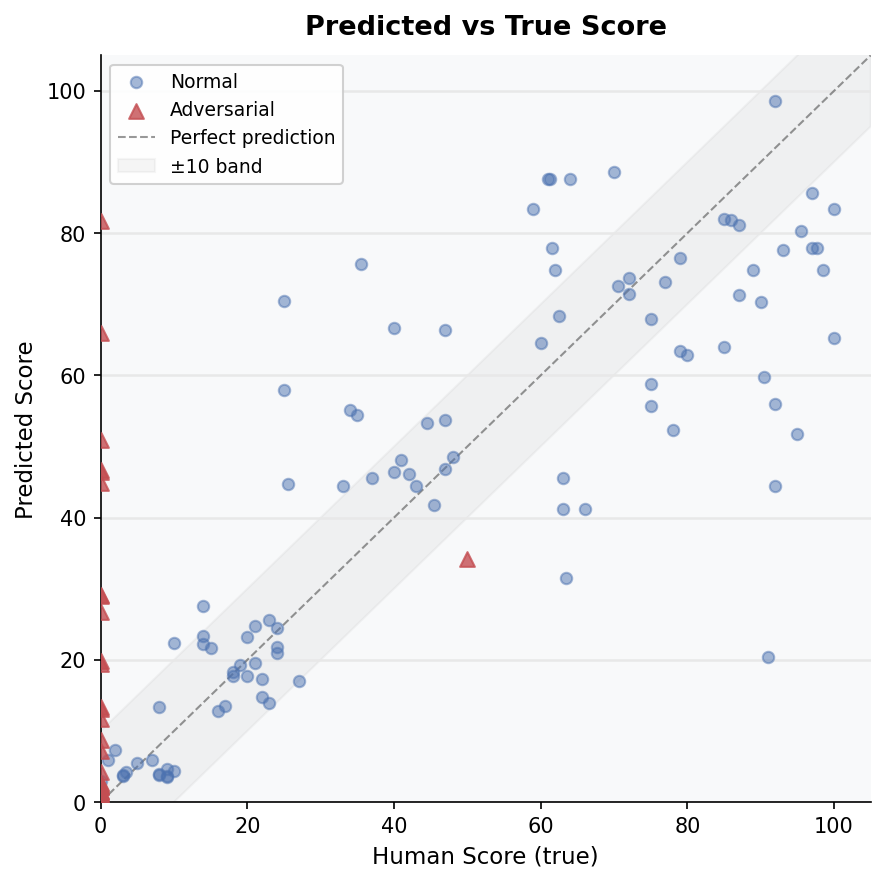
\includegraphics[width=\columnwidth]{figures/pred_vs_true_scatter.png}
\caption{Predicted vs.\ true score, single-sentence test set: normal answers (blue) and adversarial answers (red).}
\label{fig:scatter}
\end{figure}

\paragraph{Generalisation to non-templated answers.}
Table~\ref{tab:clean} trains on the original data with and without the clean
synthetic rows and tests on unseen questions; the ``clean'' rows are
clean-dataset answers to questions neither model saw. Trained on the original
data alone, the model is \emph{worse than a baseline} on natural medium
answers (Pearson 0.20 vs 0.74) and long answers (0.60 vs 0.91): it had partly
learned the templates. Adding the clean rows and the answer-slot features
raises it to 0.74 / 0.86 / 0.95. Table~\ref{tab:types} shows the remaining
errors by answer type: differently worded correct answers are still
under-scored and wrong-entity answers over-scored, though both moved in the
right direction.

\begin{table}[t]
\centering\small
\begin{tabular}{lcccc}
\toprule
Tier (rows) & Baseline & Original & +clean & +slot \\
\midrule
Single (66) & 0.41 & 0.57 & 0.65 & \best{0.74} \\
Medium (24) & 0.74 & 0.20 & 0.78 & \best{0.86} \\
Long (14) & 0.91 & 0.60 & 0.87 & \best{0.95} \\
\bottomrule
\end{tabular}
\caption{Pearson on clean-dataset answers to unseen questions: best baseline, model trained on original data only, plus clean rows, plus answer-slot features.}
\label{tab:clean}
\end{table}

\begin{table}[t]
\centering\small
\begin{tabular}{lccc}
\toprule
Answer type & Rubric & +clean & +slot \\
\midrule
Paraphrase & 95 & 54 & 67 \\
Brief (\bn{শাহজাহান।}) & 88 & 45 & 62 \\
Correct passive & 92 & 58 & 63 \\
Wrong entity & 10 & 42 & 32 \\
Wrong detail & 8 & 43 & 38 \\
\bottomrule
\end{tabular}
\caption{Mean predicted score per answer type, single-sentence clean answers to unseen questions (6 rows per type).}
\label{tab:types}
\end{table}

\paragraph{Feature importance.}
The strongest XGBoost feature is \texttt{max\_pen}, the larger of the Karak
penalty and the entity mismatch (0.34 single, 0.68 medium, 0.29 long),
followed by the negation flag on single sentences (0.24) and the Karak
penalty on long answers (0.28). The answer-slot features rank among the top
five on single-sentence answers. Graph similarity is not a top feature by
importance, and the GNN alone is the weakest single signal, yet removing it
costs 0.055 Pearson and 1.8 MAE points (Appendix~\ref{app:ablation}): it is
complementary to the sentence-level features rather than a replacement.

\section{Analysis}
\paragraph{Case studies.}
We score five answers with the trained single-sentence model.
\textbf{(1) Verb omitted.} \bn{গীতাঞ্জলি কে লিখেছিলেন?} Reference
\bn{রবীন্দ্রনাথ ঠাকুর গীতাঞ্জলি লিখেছিলেন।}, student \bn{রবীন্দ্রনাথ ঠাকুর
গীতাঞ্জলি।}: 63.4. The key answer is present (\emph{key\_match}=1, LaBSE 0.85)
but the answer is still under-scored, the remaining weakness of
Table~\ref{tab:types}. \textbf{(2) Karak reversal.} \bn{আলেকজান্ডার পোরাসকে
পরাজিত করেছেন।} vs.\ \bn{পোরাস আলেকজান্ডারকে পরাজিত করেছেন।}: LaBSE
similarity is 0.98, but the validator detects both swaps (penalty 1.0) and
the answer scores 7.1. \textbf{(3) Wrong number.} 206 vs.\ \bn{২০৭টি} bones:
21.6, from the wrong-number penalty and a missing key, without needing the
cap. \textbf{(4, 5) Negation.} \bn{সূর্য পূর্বদিকে ওঠে না।} and
\bn{ক্রিস্টোফার কলম্বাস আমেরিকা আবিষ্কার করেননি।} (fused negation) both
score 0.0; the previous version of the system scored them 72.5 and 73.3.

\paragraph{What did not work.}
Up-weighting the clean rows three times lowered performance on both clean and
original rows. Generating brief and wrong-entity training answers by rule
produced about two-thirds mislabelled rows, because the tagger marks many
common words as proper nouns, so it was dropped.

\paragraph{Earlier version of this report.}
An earlier version reported higher cross-validation scores (Pearson 0.87--0.93)
and lower adversarial performance. The former came from duplicated pairs
crossing the train/test boundary and from a GNN warm-started on the
cross-validation rows; the latter from bugs that disabled the Karak validator,
negation detection and ROUGE-L for Bengali. All numbers here use the
corrected code.

\section{Limitations and Future Work}
\paragraph{Data.} The original datasets are synthetic and templated, with
duplicated pairs and overlapping labels; the clean dataset is rubric-scored by
its authors, not by independent graders, and not yet reviewed by a native
speaker. Test sets are small (44--101 normal answers), so differences on the
non-templated medium and long subsets are not significant. The 51 adversarial
samples were inspected during development; a fresh set written by someone
who has not seen the rules would give a cleaner estimate, and synthetic
training errors share their perturbation types with it.
\paragraph{Remaining errors.} Differently worded correct answers are still
under-scored and wrong-entity answers over-scored (Table~\ref{tab:types});
correct passive paraphrases also score low; wrong locations are poorly
handled. The rule-based coreference resolver did not improve results on
these datasets (Appendix~\ref{app:ablation}).
\paragraph{Parser bottleneck.} Roles come from POS tags and case endings, so
tagger errors still choose the wrong subject. A Bengali dependency treebank
and parser, or LLM-based triple extraction, are the highest-impact next
steps; human-graded, non-templated answers are the most valuable data.

\section{Conclusion}
We presented a Bengali ASAG system that combines LaBSE similarity with a
predicate-centred knowledge graph, a Karak validator that handles case
marking and passives, sentence-aligned negation and number checks, and
answer-slot features, trained with synthetic error examples. With a
leakage-free, grouped evaluation it significantly outperforms calibrated
baselines on all three datasets (Pearson 0.83 / 0.95 / 0.91 on normal
answers) and scores role-swapped and negated answers close to zero. The
audit also shows that the original datasets reward templates, and that a
small clean dataset is needed to grade natural answers reliably.

\section*{Acknowledgements}
We thank the instructors and teaching assistants of the Introduction to NLP
course at IIIT Hyderabad for their guidance and feedback.

\small
\begin{thebibliography}{99}
\bibitem[{Bhattacharjee et~al.(2022)}]{banglabert}
Abhik Bhattacharjee, Tahmid Hasan, Wasi~Uddin Ahmad, Kazi~Samin Mubasshir, Md~Saiful Islam, Anindya Iqbal, M.~Sohel Rahman, and Rifat Shahriyar. 2022.
\newblock BanglaBERT: Language model pretraining and benchmarks for low-resource language understanding evaluation in Bangla.
\newblock In \emph{Findings of NAACL 2022}, pages 1318--1327.

\bibitem[{Chen and Guestrin(2016)}]{xgboost}
Tianqi Chen and Carlos Guestrin. 2016.
\newblock XGBoost: A scalable tree boosting system.
\newblock In \emph{Proceedings of KDD 2016}, pages 785--794.

\bibitem[{Feng et~al.(2022)}]{labse}
Fangxiaoyu Feng, Yinfei Yang, Daniel Cer, Naveen Arivazhagan, and Wei Wang. 2022.
\newblock Language-agnostic BERT sentence embedding.
\newblock In \emph{Proceedings of ACL 2022}.

\bibitem[{Horbach et~al.(2017)}]{horbach2017}
Andrea Horbach, Alexis Palmer, and Manfred Pinkal. 2017.
\newblock Finding the right prompt position for reliable short answer scoring.
\newblock In \emph{Proceedings of the 12th Workshop on Innovative Use of NLP for Building Educational Applications}, pages 1--11.

\bibitem[{Huguet~Cabot et~al.(2023)}]{mrebel}
Pere-Llu{\'i}s Huguet~Cabot, Simone Tedeschi, Axel-Cyrille Ngonga~Ngomo, and Roberto Navigli. 2023.
\newblock RED$^{\rm FM}$: a filtered and multilingual relation extraction dataset.
\newblock In \emph{Proceedings of ACL 2023}.

\bibitem[{Kipf and Welling(2017)}]{gcn}
Thomas~N. Kipf and Max Welling. 2017.
\newblock Semi-supervised classification with graph convolutional networks.
\newblock In \emph{Proceedings of ICLR 2017}.

\bibitem[{Mishra et~al.(2023)}]{indie}
Ritwik Mishra, Simranjeet Singh, Rajiv~Ratn Shah, Ponnurangam Kumaraguru, and Pushpak Bhattacharyya. 2023.
\newblock IndIE: A multilingual open information extraction tool for Indic languages.
\newblock In \emph{Findings of IJCNLP-AACL 2023}.

\bibitem[{Mohler et~al.(2011)}]{mohler2011}
Michael Mohler, Razvan Bunescu, and Rada Mihalcea. 2011.
\newblock Learning to grade short answer questions using semantic similarity measures and dependency graph alignments.
\newblock In \emph{Proceedings of ACL-HLT 2011}, pages 752--762.

\bibitem[{Nguyen et~al.(2021)}]{trankit}
Minh~Van Nguyen, Viet~Dac Lai, Amir Pouran Ben~Veyseh, and Thien~Huu Nguyen. 2021.
\newblock Trankit: A light-weight transformer-based toolkit for multilingual natural language processing.
\newblock In \emph{Proceedings of EACL 2021: System Demonstrations}.

\bibitem[{Qi et~al.(2020)}]{stanza}
Peng Qi, Yuhao Zhang, Yuhui Zhang, Jason Bolton, and Christopher~D. Manning. 2020.
\newblock Stanza: A Python natural language processing toolkit for many human languages.
\newblock In \emph{Proceedings of ACL 2020: System Demonstrations}.

\bibitem[{Riordan et~al.(2017)}]{riordan2017}
Brian Riordan, Andrea Horbach, Aoife Cahill, Torsten Zesch, and Chong~Min Lee. 2017.
\newblock Investigating neural architectures for short answer scoring.
\newblock In \emph{Proceedings of the 12th Workshop on Innovative Use of NLP for Building Educational Applications}, pages 159--168.

\bibitem[{Sultan et~al.(2016)}]{sultan2016}
Md~Arafat Sultan, Cristobal Salazar, and Tamara Sumner. 2016.
\newblock Fast and easy short answer grading with high accuracy.
\newblock In \emph{Proceedings of NAACL-HLT 2016}, pages 1070--1075.

\bibitem[{Veli{\v{c}}kovi{\'c} et~al.(2018)}]{gat}
Petar Veli{\v{c}}kovi{\'c}, Guillem Cucurull, Arantxa Casanova, Adriana Romero, Pietro Li{\`o}, and Yoshua Bengio. 2018.
\newblock Graph attention networks.
\newblock In \emph{Proceedings of ICLR 2018}.

\bibitem[{Wasi et~al.(2024)}]{banglaautokg}
Azmine~Toushik Wasi, Taki~Hasan Rafi, Raima Islam, and Dong-Kyu Chae. 2024.
\newblock BanglaAutoKG: Automatic Bangla knowledge graph construction with semantic neural graph filtering.
\newblock In \emph{Proceedings of LREC-COLING 2024}.

\bibitem[{Zhang et~al.(2019)}]{zhang2019}
Chen Zhang, Qiuchi Li, and Dawei Song. 2019.
\newblock Aspect-based sentiment classification with aspect-specific graph convolutional networks.
\newblock In \emph{Proceedings of EMNLP-IJCNLP 2019}, pages 4568--4578.
\end{thebibliography}
\normalsize

\appendix
\section{Component Ablation}\label{app:ablation}
Table~\ref{tab:ablation} removes one component at a time on the
single-sentence dataset (unseen-answer split). Features are extracted once,
the component's features are neutralised and the scorer is retrained; the
full system here is a separate training run, so it differs slightly from
Table~\ref{tab:normal} (run-to-run variation of about 0.02 Pearson).

\begin{table}[h]
\centering\small
\begin{tabular}{lcccc}
\toprule
 & \multicolumn{3}{c}{Normal answers} & Adv. \\
Variant & Pearson & MAE & F1 & MAE \\
\midrule
Full system & 0.845 & 11.89 & 84.4 & 10.55 \\
\midrule
$-$ GNN branch & 0.790 & 13.67 & 80.0 & 11.62 \\
$-$ Karak validator & 0.812 & 14.34 & 75.3 & 31.47 \\
$-$ Entity matching & 0.804 & 14.39 & 80.8 & 8.33 \\
$-$ Answer-slot features & 0.791 & 14.44 & 81.0 & 12.07 \\
$-$ Negation / number flags & 0.846 & 11.91 & 83.5 & 10.17 \\
$-$ Hard overrides & 0.845 & 11.89 & 84.4 & 10.55 \\
$-$ Synthetic training errors & 0.812 & 13.43 & 83.5 & 40.26 \\
$-$ Coreference & 0.863 & 10.17 & 86.4 & 12.07 \\
\bottomrule
\end{tabular}
\caption{Leave-one-component-out ablation, single-sentence test set (101 normal answers, 51 adversarial).}
\label{tab:ablation}
\end{table}

The GNN, Karak validator, entity matching and answer-slot features each lower
MAE on normal answers by 1.8--2.6 points. For adversarial answers the
synthetic training errors (MAE 10.6 $\rightarrow$ 40.3 without them) and the
Karak validator (31.5) are essential. The negation and number flags and the
hard overrides change little, because the Karak penalty already includes the
negation and number checks and the scorer learns these cases. Coreference
resolution does not help on this data: without it normal answers score
slightly better, while adversarial MAE rises from 10.6 to 12.1.

\section{Confusion Matrix and Adversarial Breakdown}
\begin{figure}[h]
\centering
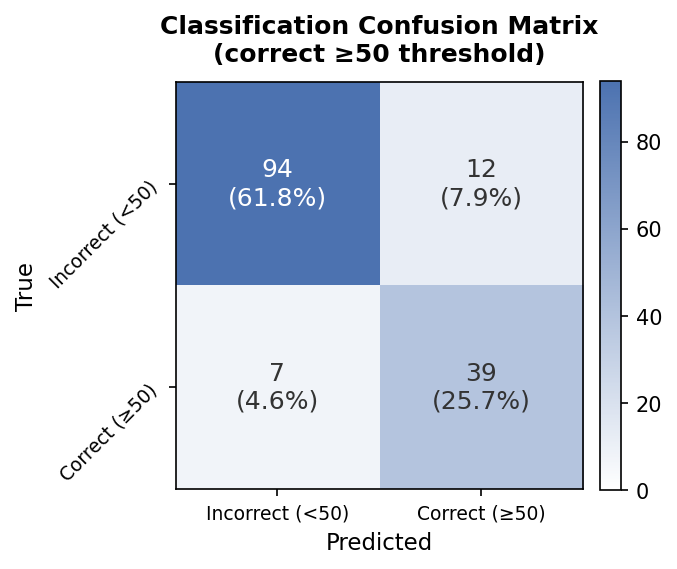
\includegraphics[width=0.85\columnwidth]{figures/confusion_matrix.png}
\caption{Pass/fail confusion matrix (score $\geq$ 50), single-sentence test set.}
\end{figure}
\begin{figure}[h]
\centering
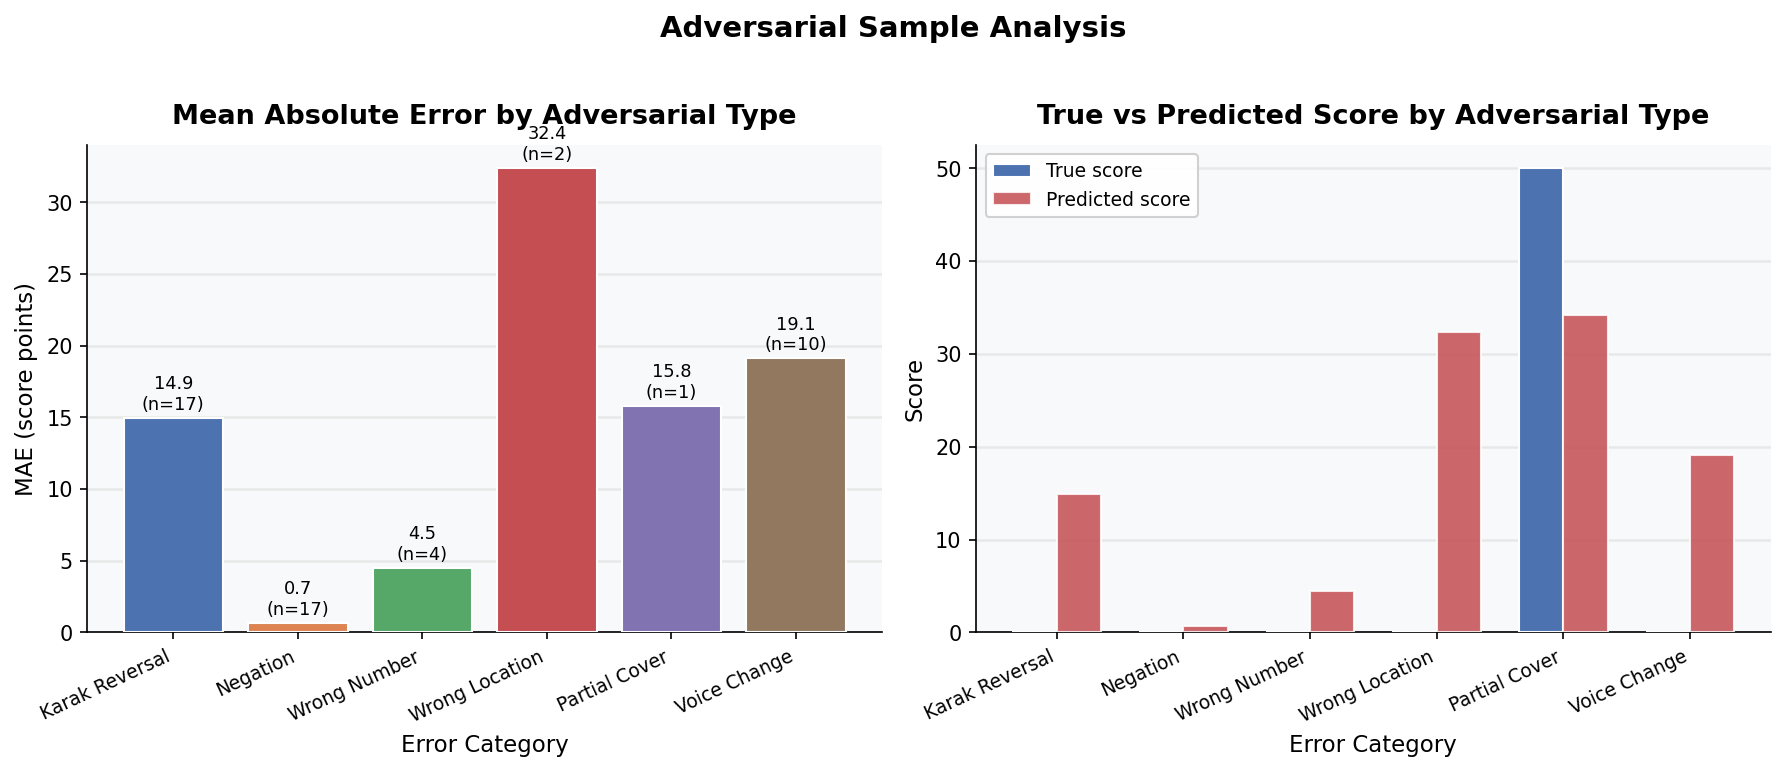
\includegraphics[width=\columnwidth]{figures/adversarial_breakdown.png}
\caption{Mean absolute error and mean predicted score per adversarial category, single-sentence test set.}
\end{figure}

\end{document}
